\chapter{Estado del arte} 
\label{chap:estadodelarte}

A pesar de ser la elección de OpenStack un requisito del proyecto, los motivos de su elección frente al resto de plataformas libres y de pago son varios. 

En este capítulo vamos a proceder a describir los servicios y características \textit{cloud} que ofrecen algunos de los proveedores de servicio IaaS principales y justificaremos la elección de OpenStack haciendo una pequeña comparativa.

También veremos algunas de las empresas más fuertes que ofrecen un servicio de computación en la nube basado en OpenStack para a continuación justificar la vía por la que optaremos.

Para finalizar el capítulo veremos algunos datos que nos darán una clara imagen de la importancia de OpenStack en los despliegues de IT y el panorama TIC actual.

\section{Plataformas de Cloud Computing}
Al desplegar un proyecto de IaaS pretendiendo crear nuestra propia nube, inmediatamente se nos vienen a la cabeza proveedores de servicio de pago como Amazon Web Services, Rackspace Cloud Server, Mirantis, Microsoft Windows Azure, VMware o Google Cloud. 

Existen otros proveedores que ofrecen plataformas open source como es el caso de Eucalyptus, OpenNebula o CloudStack.

Sin mas dilación, vamos a ver las características principales de algunos de estos proveedores (dos de pago y dos open source) los cuales hemos elegido por su relevancia dentro de los servicios \textit{cloud}.

\subsection{Amazon Web Services}

\begin{figure}
    \centering
    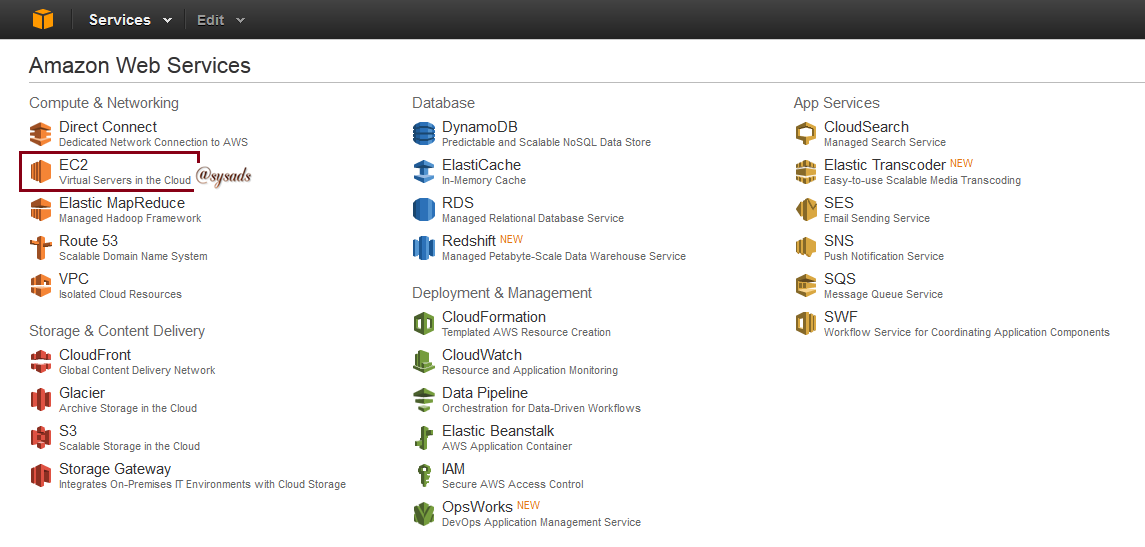
\includegraphics[width=0.7\textwidth]{imagenes/capitulo2/amazon.png}
    \caption{Panel de control de Amazon Web Services.}
	\vspace{0.3cm}
    \footnotesize{Fuente: Amazon}
    \label{amazon}
\end{figure}

Amazon Elastic Compute Cloud (Amazon EC2) es un servicio web que proporciona capacidad informática con tamaño modificable en la nube. Está diseñado para facilitar a los desarrolladores recursos informáticos escalables vía web a través de una sencilla interfaz cuyo panel de control podemos ver en la Fig.\ref{amazon}. Según la propia empresa ofrecen \cite{noauthor_aws_nodate}:

\begin{itemize}
\item Reducción del tiempo necesario para obtener y arrancar nuevas instancias de un servidor en minutos, lo que permite escalar rápidamente la capacidad, ya sea aumentándola o reduciéndola, según cambien sus necesidades.
\item Modelo económico consecuente. Pago sólo por la capacidad que se utiliza realmente.
\item Amazon EC2 proporciona a los desarrolladores las herramientas necesarias para crear aplicaciones resistentes a errores y para aislarse de los casos de error más comunes.
\item Compatibilidad con otros servicios de AWS.
\item Fiabilidad. El servicio se ejecuta en los centros de datos e infraestructura de red acreditados de Amazon.
\item Seguridad. Mecanismos de VPC, listas de acceso, VPN IPsec e instancias aisladas.
\item Asequibilidad. Amazon EC2 ofrece ventajas financieras dentro su corporación.
\end{itemize}

\subsection{VMware}
VMware es una compañía suministradora de servicios de virtualización por software donde las máquinas virtuales proporcionan un ambiente de ejecución similar, a todos los efectos, a un computador físico. Entre sus servicios de virtualización ofrece \cite{noauthor_virtualizacion_nodate}:

\begin{itemize}
\item Virtualización de servidores.
\item Virtualización de redes.
\item Virtualización de escritorios.
\item Virtualización de aplicaciones.
\item Virtualización de almacenamiento.
\end{itemize}

\subsection{VMware vSphere}
Dentro de las opciones que nos brinda VMware cabe destacar VMware vSphere, diseñado para organizaciones que desean optimizar los activos de infraestructura
tecnológica existentes y demorar las costosas expansiones del centro de datos,
\textit{VMware® vSphere® Standard Edition} proporciona una solución de consolidación básica de las aplicaciones, a fin de reducir drásticamente los costes de hardware, además de acelerar la implementación de las aplicaciones sin tener que programar ningún tiempo de inactividad.

VMware vSphere permite a los usuarios ejecutar aplicaciones críticas para el negocio con confianza y responder con mayor rapidez a las necesidades empresariales acelerando el cambio hacia la computación en la nube para los centros de datos.

Esta herramienta ofrece una serie de servicios \cite{noauthor_vmware-vsphere-datasheet.pdf_nodate} como vemos en la Fig.\ref{VMware} que la dotan de ventajas entre las que destacamos:

\begin{itemize}
\item Mayor eficiencia gracias a la automatización y mejora del rendimiento del hardware pasando del 15 al 80\% de utilización.
\item Disminución de gastos de propiedad y operativos.
\item Escalabilidad y disponibilidad.
\item Plataforma basada en estándares.
\end{itemize}

\begin{figure}
    \centering
    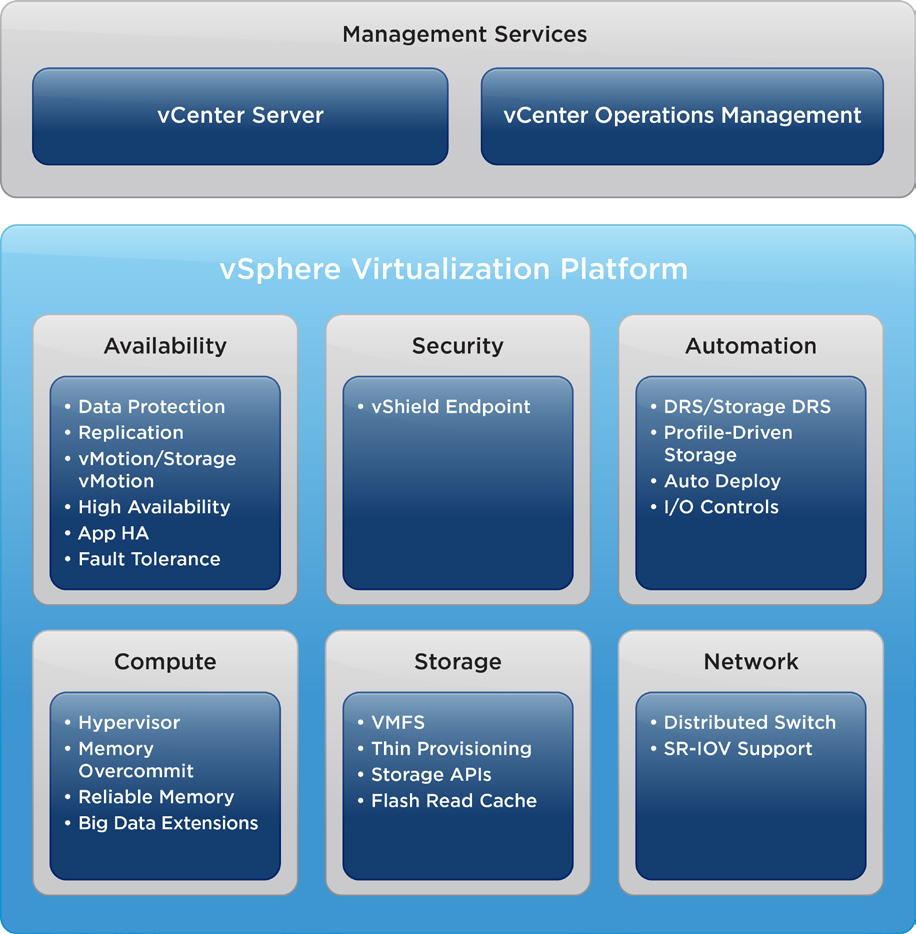
\includegraphics[width=0.7\textwidth]{imagenes/capitulo2/VMware.png}
    \caption{Servicios de VMware vSphere.}
	\vspace{0.3cm}
    \footnotesize{Fuente: VMware}
    \label{VMware}
\end{figure}

\subsection{Apache CloudStack}
Apache CloudStack es un proyecto de alto nivel de la Fundación de Software
Apache. El proyecto desarrolla software de código abierto y nubes con infraestructura
como servicio (IaaS).
Este proyecto provee las herramientas necesarias para entregar nubes públicas de
manera fiable y escalable.
Entre sus características se encuentran las siguientes \cite{noauthor_apache_nodate}:

\begin{itemize}
\item Trabaja con hipervisores como Xen, KVM, HyperfV o Vmware ESXiconVsphere.
\item Provee una interfaz sencilla para el manejo de toda la operativa de un
IaaS por medio de  una interfaz visual o de comandos.
\item Tiene una API Nativa.
\item Compatibilidad con Amazon S3 y EC2.
\item Maneja almacenamiento para instancias basado en los hipervisores
además de plantillas, capturas de instancias e Imágenes ISO como
almacenamiento secundario.
\item Servicios de redes desde la capa de enlace a la de aplicación como por ejemplo: DHCP, NAT, cortafuegos y VPNs.
\item Está separada en partes: Red, cómputo y almacenamiento.
\item Soporte multi-usario o multi-tenant: a un proyecto pueden acceder varios usuarios concurrentemente.
\end{itemize}

\subsection{OpenNebula}
OpenNebula surge como un proyecto de investigación llevado a cabo desde la Universidad Complutense de Madrid. Esta enfocado en la computación distribuida, virtualización y plataformas IaaS bajo una licencia Apache 2.0.\cite{noauthor_about_nodate}

Esta plataforma esta dotada con algunas funcionalidades que convierten a OpenNebula en un gestor de VDC (Virtual Data Center) con el que encargarse desde la capa más básica de red y almacenamiento, hasta los procesos de gestión de usuarios, tiempos de uso, explotación de recursos y escalabilidad:

\begin{itemize}
\item Gestión de recursos flexible y despliegue de máquinas pre-configuradas.
\item Gestión de usuarios: uso, facturación, provisionamiento.
\item Gestión de perfiles de seguridad.
\item Gestión de redes.
\item Gestión de almacenamiento.
\item Mecanismos de alta disponibilidad y clusters.
\item Creación de virtual centers, zonas o nubes híbridas.
\item Aplicaciones en Market App.
\item Servicios de monitorización. 
\item API para integración.
\item Sistema de Hooks.
\item Compatible con hipervisores Xen, KVM, QUEMU, VMWare ESXI, ESX Server.
\end{itemize}

\subsection{Comparativa de las plataformas Cloud de pago con OpenStack}

El principal motivo de la elección de OpenStack frente a otras plataformas de pago como VMware o AWS, es precisamente el económico. La filosofía del proyecto es que se realice mediante una plataforma cloud de software libre apta para la investigación. 

Además OpenStack cuenta con todos los servicios que estas plataformas de pago ofrecen. La principal diferencia radica en el hecho de que las plataformas de pagos ofrecen sus propia infraestructura y el despliegue y uso es mucho más sencillo e intuitivo. Basta con contratar aquellos servicios que queramos y estos serán administrados por nosotros.

Esto no es obviamente algo que deseemos pues el objetivo de nuestro proyecto es realizar el despliegue de nuestra propia infraestructura y adaptarla a aquellos recursos y servicios que queramos y de los que podamos disponer.

\subsection{Comparativa de las plataformas Cloud open source con OpenStack}

Eucalyptus, OpenNebula y CloudStack, son los principales competidores a la hora de realizar nuestra elección frente a OpenStack. 

El primer caso, Eucalyptus, si ni quiera existe ya hoy en día, razón por la cuál no hemos hablado de dicho proyecto.

Con respecto a OpenNebula y CloudStack, una característica fundamental para tomar la decisión se representa en la Fig.\ref{comparativa cloud open source} extraída de la web de OpenNebula \cite{noauthor_eucalyptus_nodate} donde podemos ver una comparativa de las distintas herramientas en función de dos criterios:

\begin{itemize}
\item El modelo de cloud:
\begin{itemize}
\item Virtualización del centro de datos. Entender la nube como una extensión de la virtualización en el centro de datos.
\item Provisión de infraestructura: Herramienta de aprovisionamiento para suministrar recursos virtualizados según demanda.
\end{itemize}
\item La flexibilidad.
\end{itemize}

\begin{figure}
    \centering
    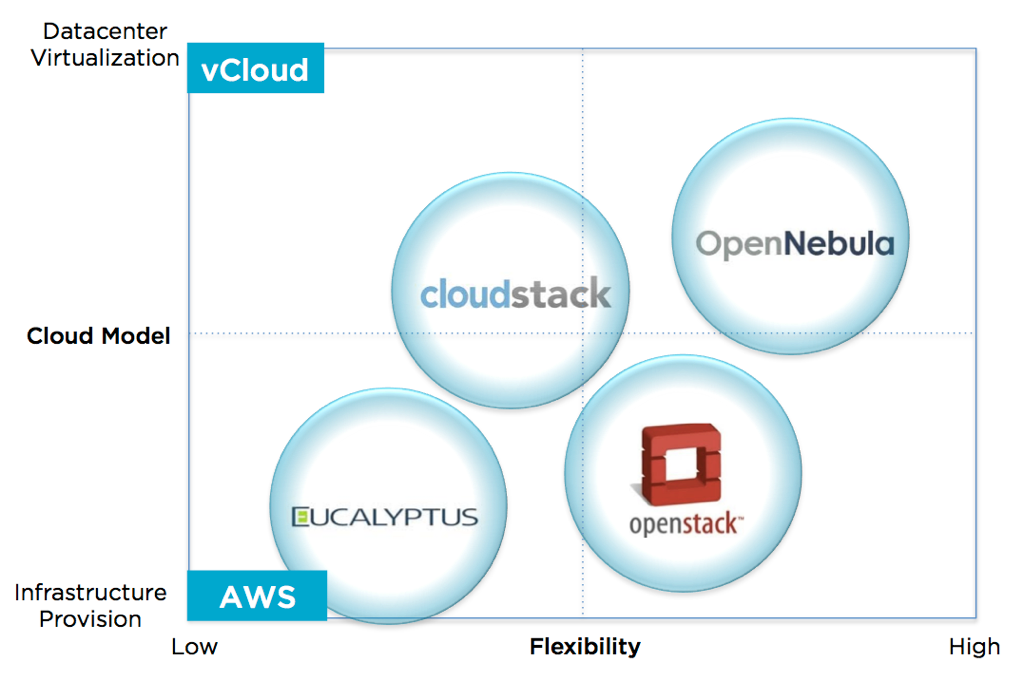
\includegraphics[width=0.7\textwidth]{imagenes/capitulo2/comparativaCloudPublica.png}
    \caption{Comparativa entre clouds open source en función del uso y la flexibilidad.}
	\vspace{0.3cm}
    \footnotesize{Fuente: Ignacio M.Llorente, “Eucalyptus, CloudStack, OpenStack and OpenNebula: A Tale of Two Cloud Models", OpenNebula, 2013}
    \label{comparativa cloud open source}
\end{figure}

Cómo vemos, OpenStack se postula como la plataforma más flexible para construir nuestra IaaS. Además, posee todas las características de sus competidores incorporando una actualización constante de los proyectos que forman parte de esta herramienta y que podemos incorporar a nuestro proyecto de forma modular en función de nuestras necesidades.

Para acabar la comparación, un estudio realizado en 2013 por Qingye Jiang \cite{qingye_jiang_cy12-q4_2013} en el que hace una comparativa de estas cuatro plataformas, ya mostraba la clara tendencia de comunidad, empresas y desarrolladores a usar OpenStack. En la Fig.\ref{comparativa del chino} vemos una extracción del estudio en el que se aprecia el número de participantes mensual en los proyectos y como OpenStack irrumpió desde un inicio tomando clara ventaja al resto de soluciones.

\begin{figure}
    \centering
    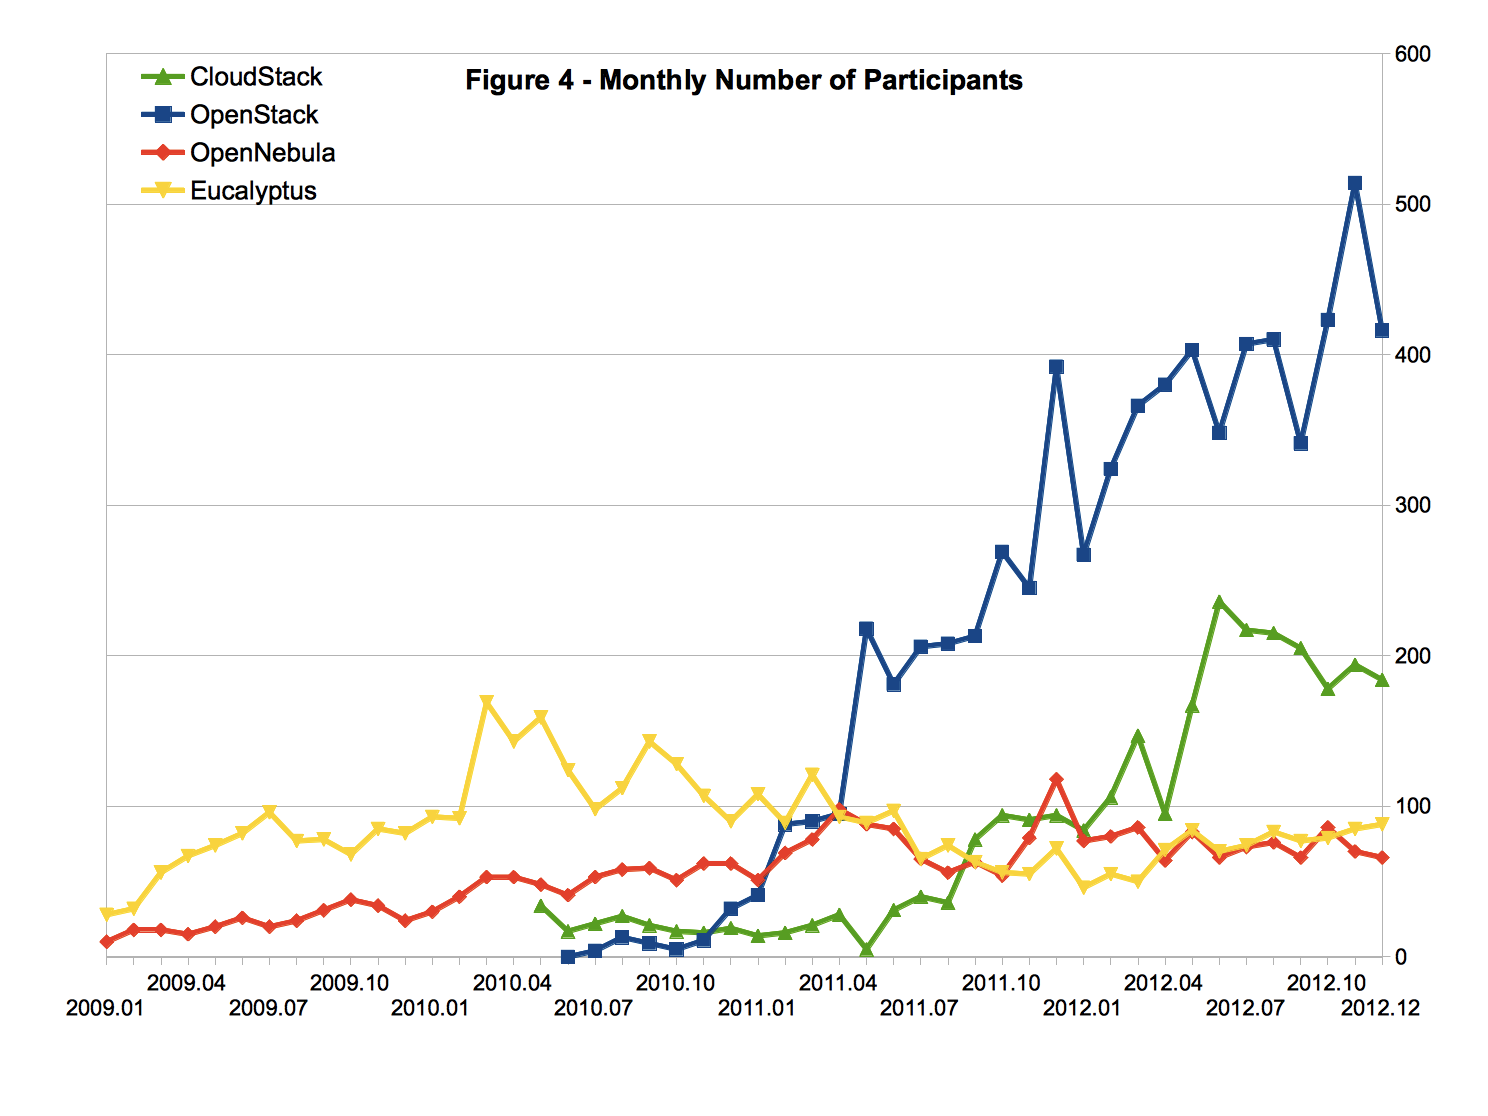
\includegraphics[width=0.7\textwidth]{imagenes/capitulo2/mesOpenStack.png}
    \caption{Número de participantes mensual.}
	\vspace{0.3cm}
    \footnotesize{Fuente: Qingye Jiang, “OpenStack vs OpenNebula vs Eucalyptus vs CloudStack", Open Source IaaS Community Analysis, 2013}
    \label{comparativa del chino}
\end{figure}


\section{Vendedores de OpenStack}
Son varios los proveedores que ofrecen sus productos y servicios junto con OpenStack. Estos proveedores abarcan desde distribuidores de hipervisores con estrecha integración a su plataforma hasta proveedores en la nube que ofrecen versiones de cloud públicas, privadas o híbridas. En lo que sigue de la sección, nombraremos algunas de las más representativas del mercado \cite{shrivastwa_vendor_2016}.

\subsection{VMware Integrated OpenStack}

De esta solución podemos destacar:

\begin{itemize}
\item VMware Integrated OpenStack viene con un proveedor de hipervisores. 
\item Se  puede obtener de forma gratuita con una licencia enterprise plus de VMware.
\item Se integra muy bien en el cliente web vSphere y despliega un OpenStack enfocado a un entorno productivo en solo unos pocos clics.
\item Está estrechamente integrado con el ESXi Hypervisor. 
\item La última versión integrada es \textit{Kilo}.
\end{itemize}


Su popularidad radica en el hecho de que existen muchas empresas que ya han hecho una inversión considerable en términos de licencias de VMware para hipervisores \cite{noauthor_integrated_nodate}.

\subsection{Rackspace Cloud}
Rackspace necesita una mención especial, no solo porque ejecutan una famosa nube pública basada en OpenStack, sino también porque si no fuera por ellos, ni siquiera tendríamos OpenStack ya que fueron Rackspace y NASA los que comenzaron este proyecto en 2010. Sin embargo, todavía están en la versión \textit{Icehouse} con el hipervisor Xen \cite{noauthor_choosing_nodate}.

\subsection{HP Helion}
En el segmento de software libre y  código abierto (FOSS) para productos en la nube, OpenStack y Eucalyptus fueron dos productos que resolvieron los mismos problemas. HP adquirió Eucalyptus y lo ha agregó a sus ofertas en la nube de Helion. Actualmente incorpora también OpenStack pudiendo elegir entre ambas opciones \cite{noauthor_software_nodate}.

\subsection{Cisco OpenStack}
Cisco tiene una distribución OpenStack que se ejecuta en su chasis y proporciona soluciones en la nube, en su mayoría privadas, para las empresas que permiten una fácil implementación de una instalación compatible con OpenStack en sus centros de datos \cite{noauthor_cisco_nodate}.

\subsection{Mirantis OpenStack}
Mirantis OpenStack es uno de los más flexibles y al mismo tiempo, una distribución abierta de OpenStack que además ofrece servicio de soporte técnico.

En cuanto a los hipervisores, se abarca desde Xen, Docker, Hyper-V, ESXi, LXC (contenedores Linux), QEMU y KVM. Por lo tanto, si se desean opciones más respaldadas en términos de hipervisores, esta será la elección ideal \cite{noauthor_mirantis_nodate}.

\subsection{SwiftStack}
SwiftStack es un ejemplo de implementación parcial de OpenStack. Solo implementa como su nombre lo indica, Swift, el servicio de almacenamiento de objetos de OpenStack \cite{noauthor_swiftstack_nodate}.

\subsection{IBM Cloud Manager}
El administrador de IBM Cloud pertenece al gigante tecnológico IBM, que proporciona integración con el hipervisor z/VM ejecutándose en mainframes. También proporciona conjuntos de herramientas de gestión junto con su distribución. Su lanzamiento actual se basa en \textit{Juno} \cite{peterson2700042wjc_ibm_2009}.

\subsection{Suse Cloud}
Basada en OpenStack y Crowbar, esta oferta de nube privada admite implementaciones mixtas de hipervisor en la nube basadas en la versión de OpenStack de \textit{Icehouse} \cite{noauthor_suse_nodate}.

\subsection{Sobre los vendedores}
De nuevo, a la hora de implementar nuestra IaaS, no vamos a optar por ninguno de los vendedores citados sino que, partiendo de la instalación de Ubuntu Server en nuestros servidores, realizaremos nuestro propio despliegue por varios motivos:

\begin{itemize}
\item El primero vuelve a ser el económico. Como proyecto de investigación y prueba de concepto que estamos realizando, la barrera económico es clave en el desarrollo del proyecto.
\item Todas las soluciones citadas dan soporte sólo a algunos de los proyectos que forman OpenStack. De este modo, proyectos menos conocidos o usados por su naturaleza, como el caso de Tacker, no tendrían cabida. Además, así podremos incorporar sólo aquellos proyectos que nos ayuden a cumplir nuestros objetivos.
\item Otro motivo es la naturaleza académica del proyecto. Realizando nuestro propio despliegue alcanzaremos un conocimiento mucho más profundo acerca de los aspectos relativos al despliegue de una nube IaaS.
\item Por último, la mayoría de distribuidores se basan en versiones de OpenStack que ya no tiene soporte. En nuestro caso elegiremos para el desarrollo Queens, que es la última versión estable \cite{noauthor_releases:_nodate} del proyecto e incorpora actualizaciones de todos los servicios y proyectos de OpenStack. 
\end{itemize}



\section{El papel de OpenStack en el ámbito IT}

El proyecto OpenStack surge de la colaboración global de desarrolladores tecnológicos y de computación en la nube que crearon esta plataforma. Cientos de las marcas más grandes del mundo incluyendo AT\&T, Bloomberg, Best Buy, Comcast, eBay, PayPal, SAP, Time Warner Cable, Verizon, Visa, Walmart, Wells Fargo y Yahoo, por nombrar algunos, confían en OpenStack para el funcionamiento diario de sus negocio, reduciendo costos y ganando en movilidad. 

\begin{figure}
    \centering
    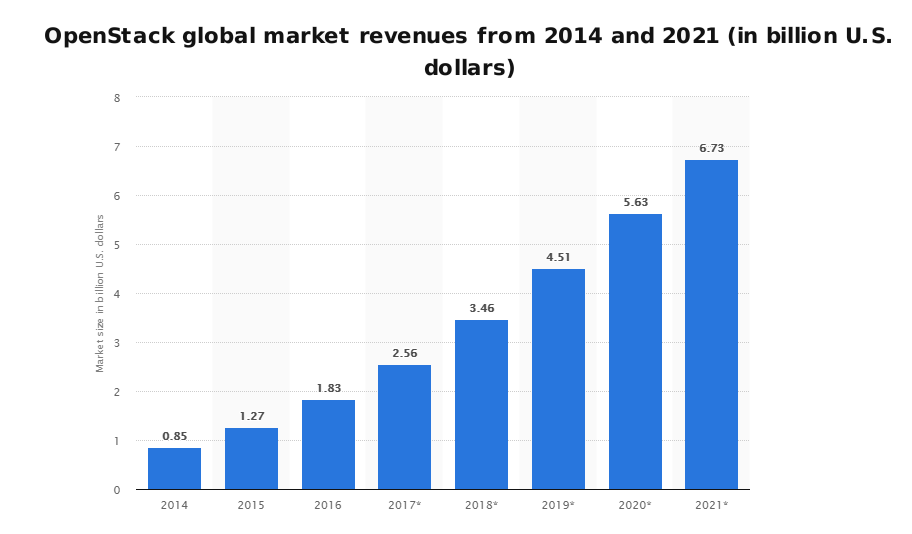
\includegraphics[width=0.7\textwidth]{imagenes/capitulo2/ganancias_OpenStack.png}
    \caption{Ingresos globales de mercado de OpenStack de 2014 a 2021 en miles de millones de dólares estadounidenses
.}
	\vspace{0.3cm}
    \footnotesize{Fuente: Statista}
    \label{ganancias_OpenStack}
\end{figure}

OpenStack es utilizado por el 50\% de la lista de las compañías que más ingresos generan en EE.UU. conocida como \textit{US Fortune 100} \cite{noauthor_fortune_nodate}, que abarca industrias que incluyen todo tipo de servicios, finanzas, fabricación, medios de comunicación, investigación, gubernamental, universitarios, venta minorista, tecnología y telecomunicaciones. Para mostrar este hecho en términos económicos, en la Fig.\ref{ganancias_OpenStack} se muestra un estudio del portal de estadísticas \textit{Statista} \cite{noauthor_statistic_nodate} donde se estima que las ganancias que generará la plataforma solo este año serán de aproximadamente 3.46 billones de dólares americanos con una tendencia anual creciente.


OpenStack está basado en estándares abiertos.  Uno de los principales elementos de OpenStack es la API abierta (\textit{Application Program Interface}), que es un conjunto de definiciones de rutina, protocolos y herramientas para crear software y aplicaciones. Debido a que la API OpenStack está tan bien desarrollada, atrae a los desarrolladores, facilitando su trabajo.


Lanzado en 2010, el proyecto OpenStack, cuenta con una de las comunidades de código abierto de más rápido crecimiento en el mundo, está respaldado por una comunidad vibrante de desarrolladores y algunos de los nombres más grandes en la industria. Hasta la fecha, posee una contribución de más de 20 millones de líneas de código por más de 90000 personas y 600 empresas en 185 países. En la Fig.\ref{Alcance de OpenStack} podemos ver un resumen de las dimensiones del proyecto hasta la fecha.

\begin{figure}
    \centering
    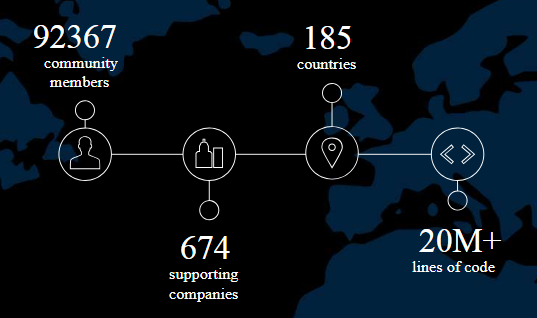
\includegraphics[width=0.7\textwidth]{imagenes/capitulo2/community.png}
    \caption{Alcance de OpenStack.}
	\vspace{0.3cm}
    \label{Alcance de OpenStack}
\end{figure}

Por tanto, el hecho de ser una plataforma open source unido a que es la herramienta más usada para entornos cloud en la actualidad y la que cuenta con la mayor comunidad en su ámbito y un número enorme de empresas contribuidoras fundamentales en cualquier desarrollo tecnológico de hoy día, hace que la elección sea sencilla.

\subsection{Casos de éxito}

OpenStack es el producto de nube más exitoso, las implementaciones con él son demasiadas para detallarlas. En esta sección, veremos algunos de los casos de uso más comunes donde se puede ver OpenStack en acción.\cite{shrivastwa_openstack_2015}

\begin{itemize}
\item \textbf{Enterprise Private Cloud}. Uno de los casos de uso más comunes si nos encontramos en la organización de IT de cualquier empresa que opte por ofrecer una nube privada a sus diferentes unidades de negocios, que ahora demandan agilidad, flexibilidad y menor tiempo de lanzamiento al mercado, es sin duda OpenStack.

Algunas de las empresas que lo han adoptado son eBay, Alcatel-Lucent, BMW, PayPal, NASA y Sony, entre otras.

\item \textbf{Proveedores de servicio}. Si miramos líneas de negocio de proveedores de servicios, como un proveedor de centro de datos, es posible que este desee comenzar a ofrecer servicios en la nube. La naturaleza distribuida de OpenStack puede ayudarlo a crear una nube con el fin de proveer del servicio de un centro de datos virtualizado a sus usuarios, agregando algunas integraciones adicionales por encima de la oferta estándar de OpenStack, como conjuntos de herramientas y SLA.

Hay varios proveedores de servicios que usan OpenStack hoy como AT \& T, Telstra, CCS (Cisco Cloud Services), Korea Telecom, Dream Host, y más.

\item\textbf{Escuelas / Centros de investigación}. Incluso las escuelas usan OpenStack en sus laboratorios para proporcionar rápidamente diferentes tipos de cargas de trabajo para los estudiantes, el personal y los profesores de investigación que están llevando a cabo proyectos o investigando en varios campos de su estudio. No depender del equipo de IT reduce en gran medida el tiempo requerido para comenzar un proyecto.

Algunos de los ejemplos notables son CERN, MIT, CSAIL, etc.

\item \textbf{Proveedores web, SaaS}. Este tipo de empresas necesitan agilidad. Hay varios cientos de ellos y sus criterios de éxito dependen de cuán rápido puedan incorporar nuevas características a sus productos, por lo tanto, el Dev / Test y todo el paradigma DevOps para ellos se convierte en la clave para la supervivencia y OpenStack puede ayudarlos a lograrlo. Estas compañías inevitablemente usan OpenStack o un equivalente para abordar esta tarea.

Algunos ejemplos en este segmento serían MercadoLibre.com o Platform 9.
\end{itemize}

